\begin{figure}
    \centering
    \begin{subfigure}{0.48\linewidth}
        \centering
        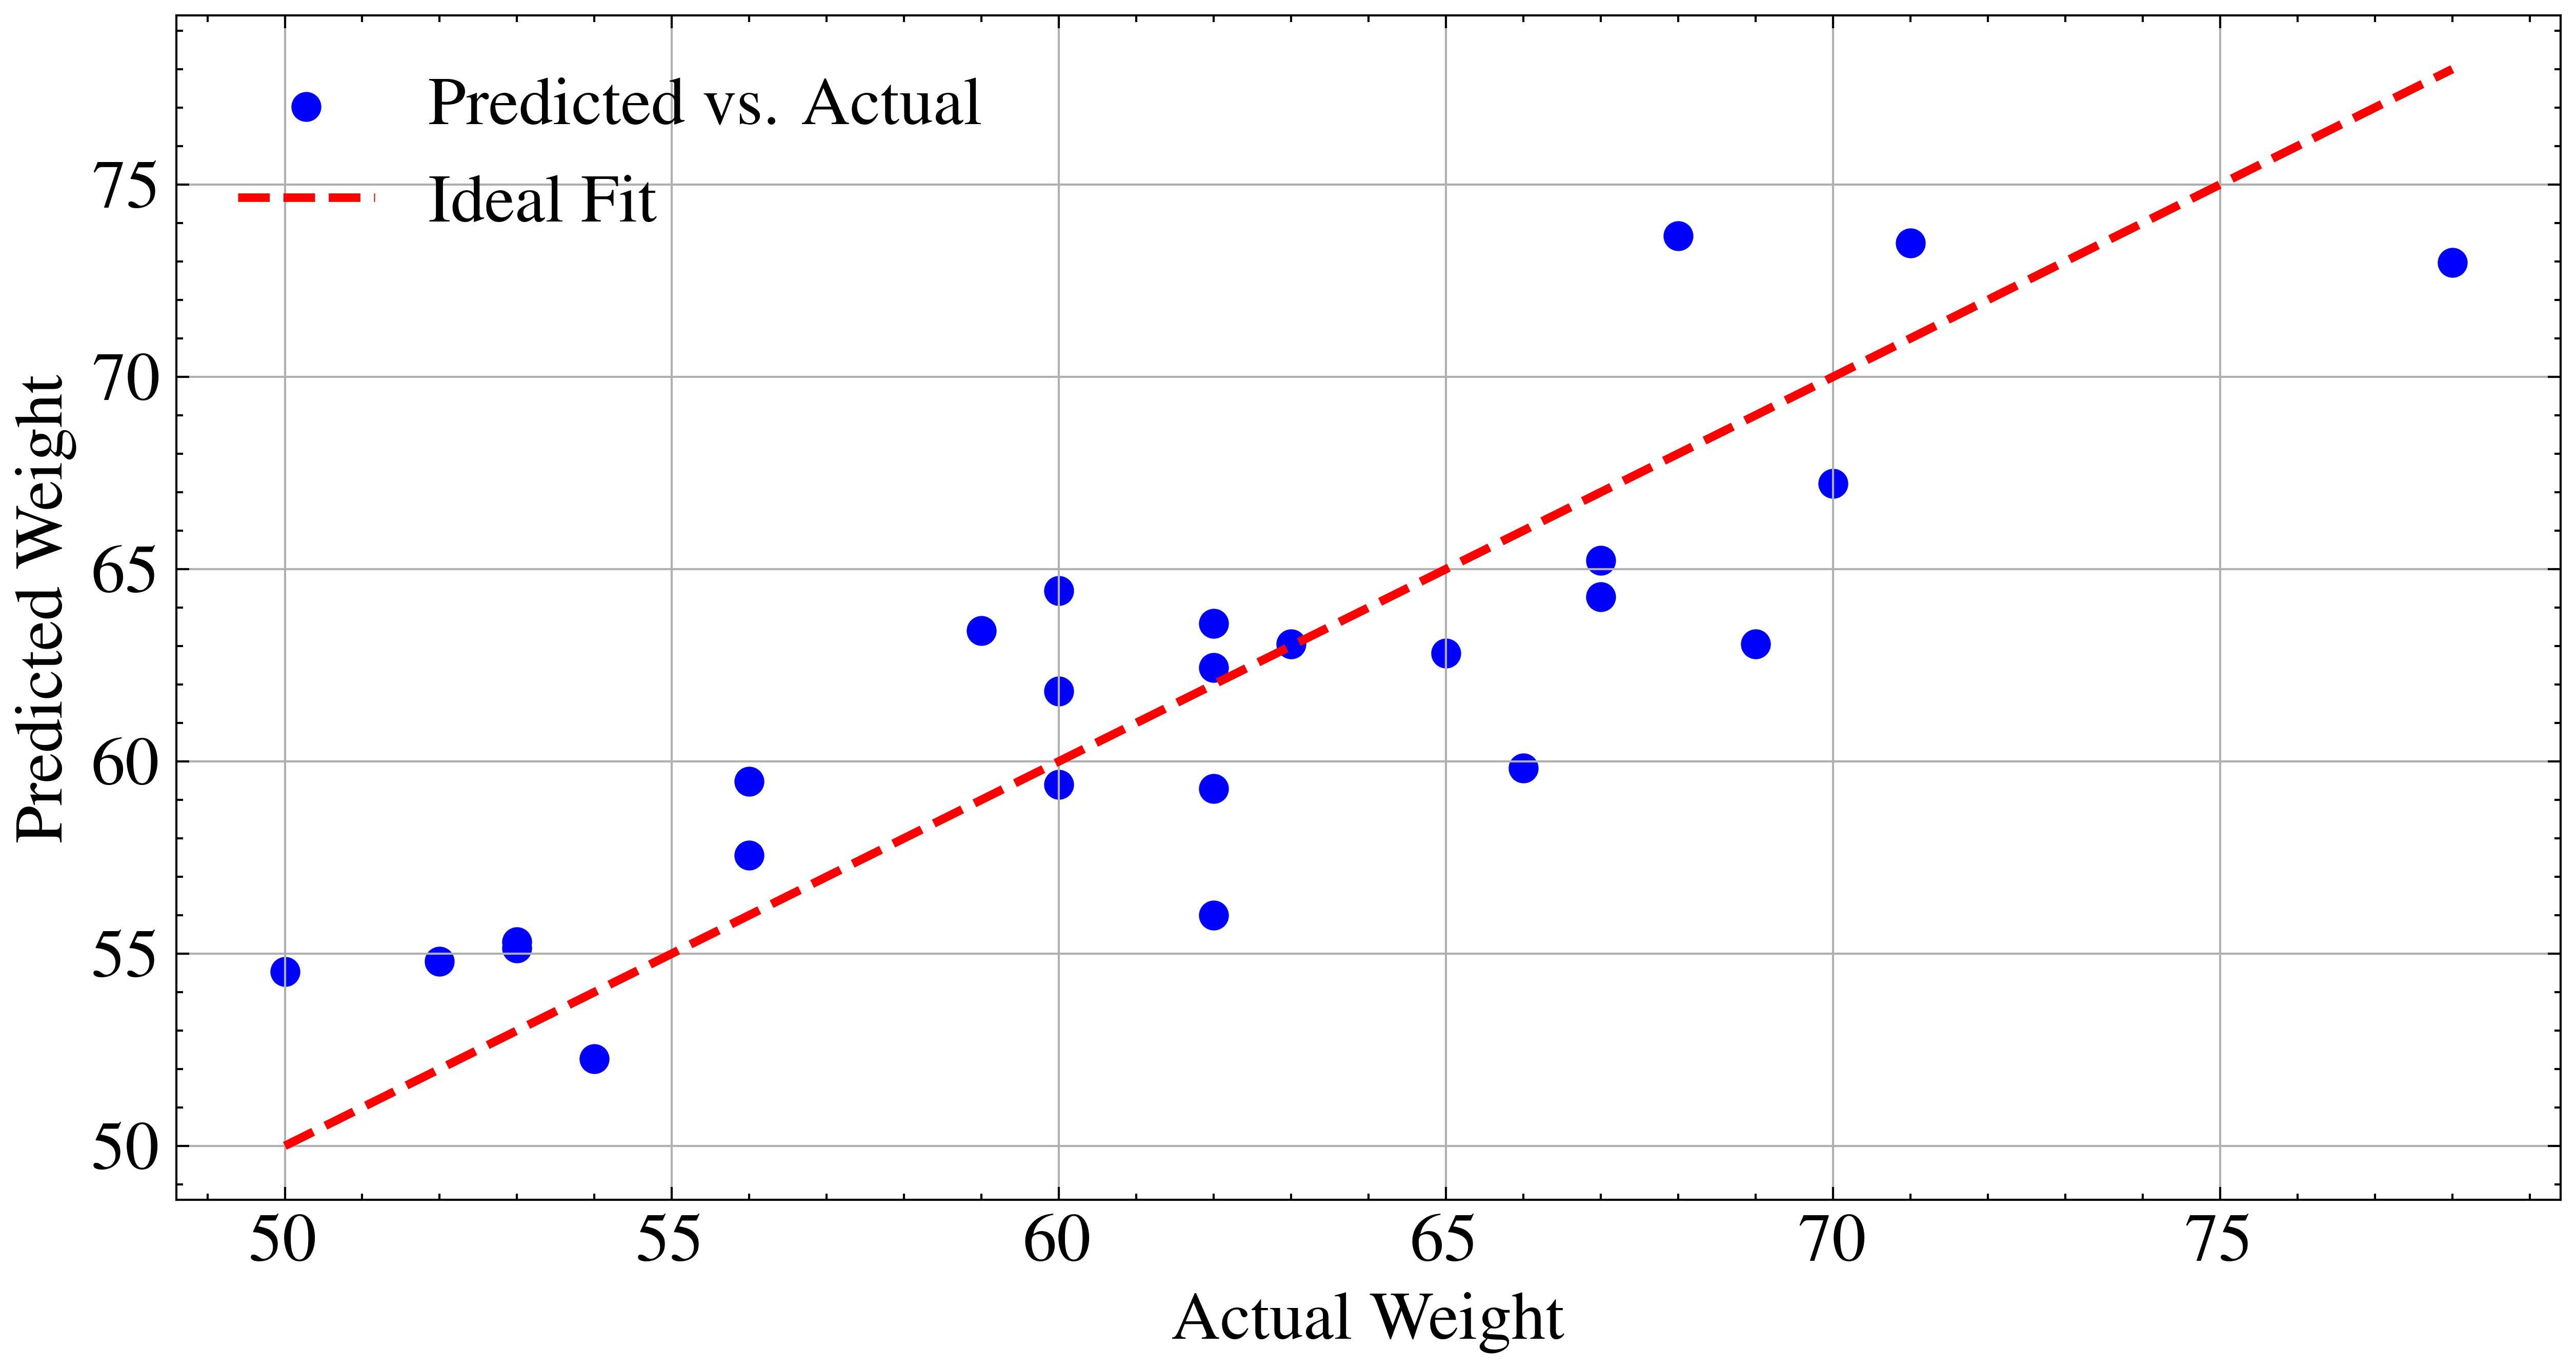
\includegraphics[width=\linewidth]{src/figures/polynominal-regression/polynomial_regression-n-1.png}
        \subcaption{$n=1$}
    \end{subfigure}
    \begin{subfigure}{0.48\linewidth}
        \centering
        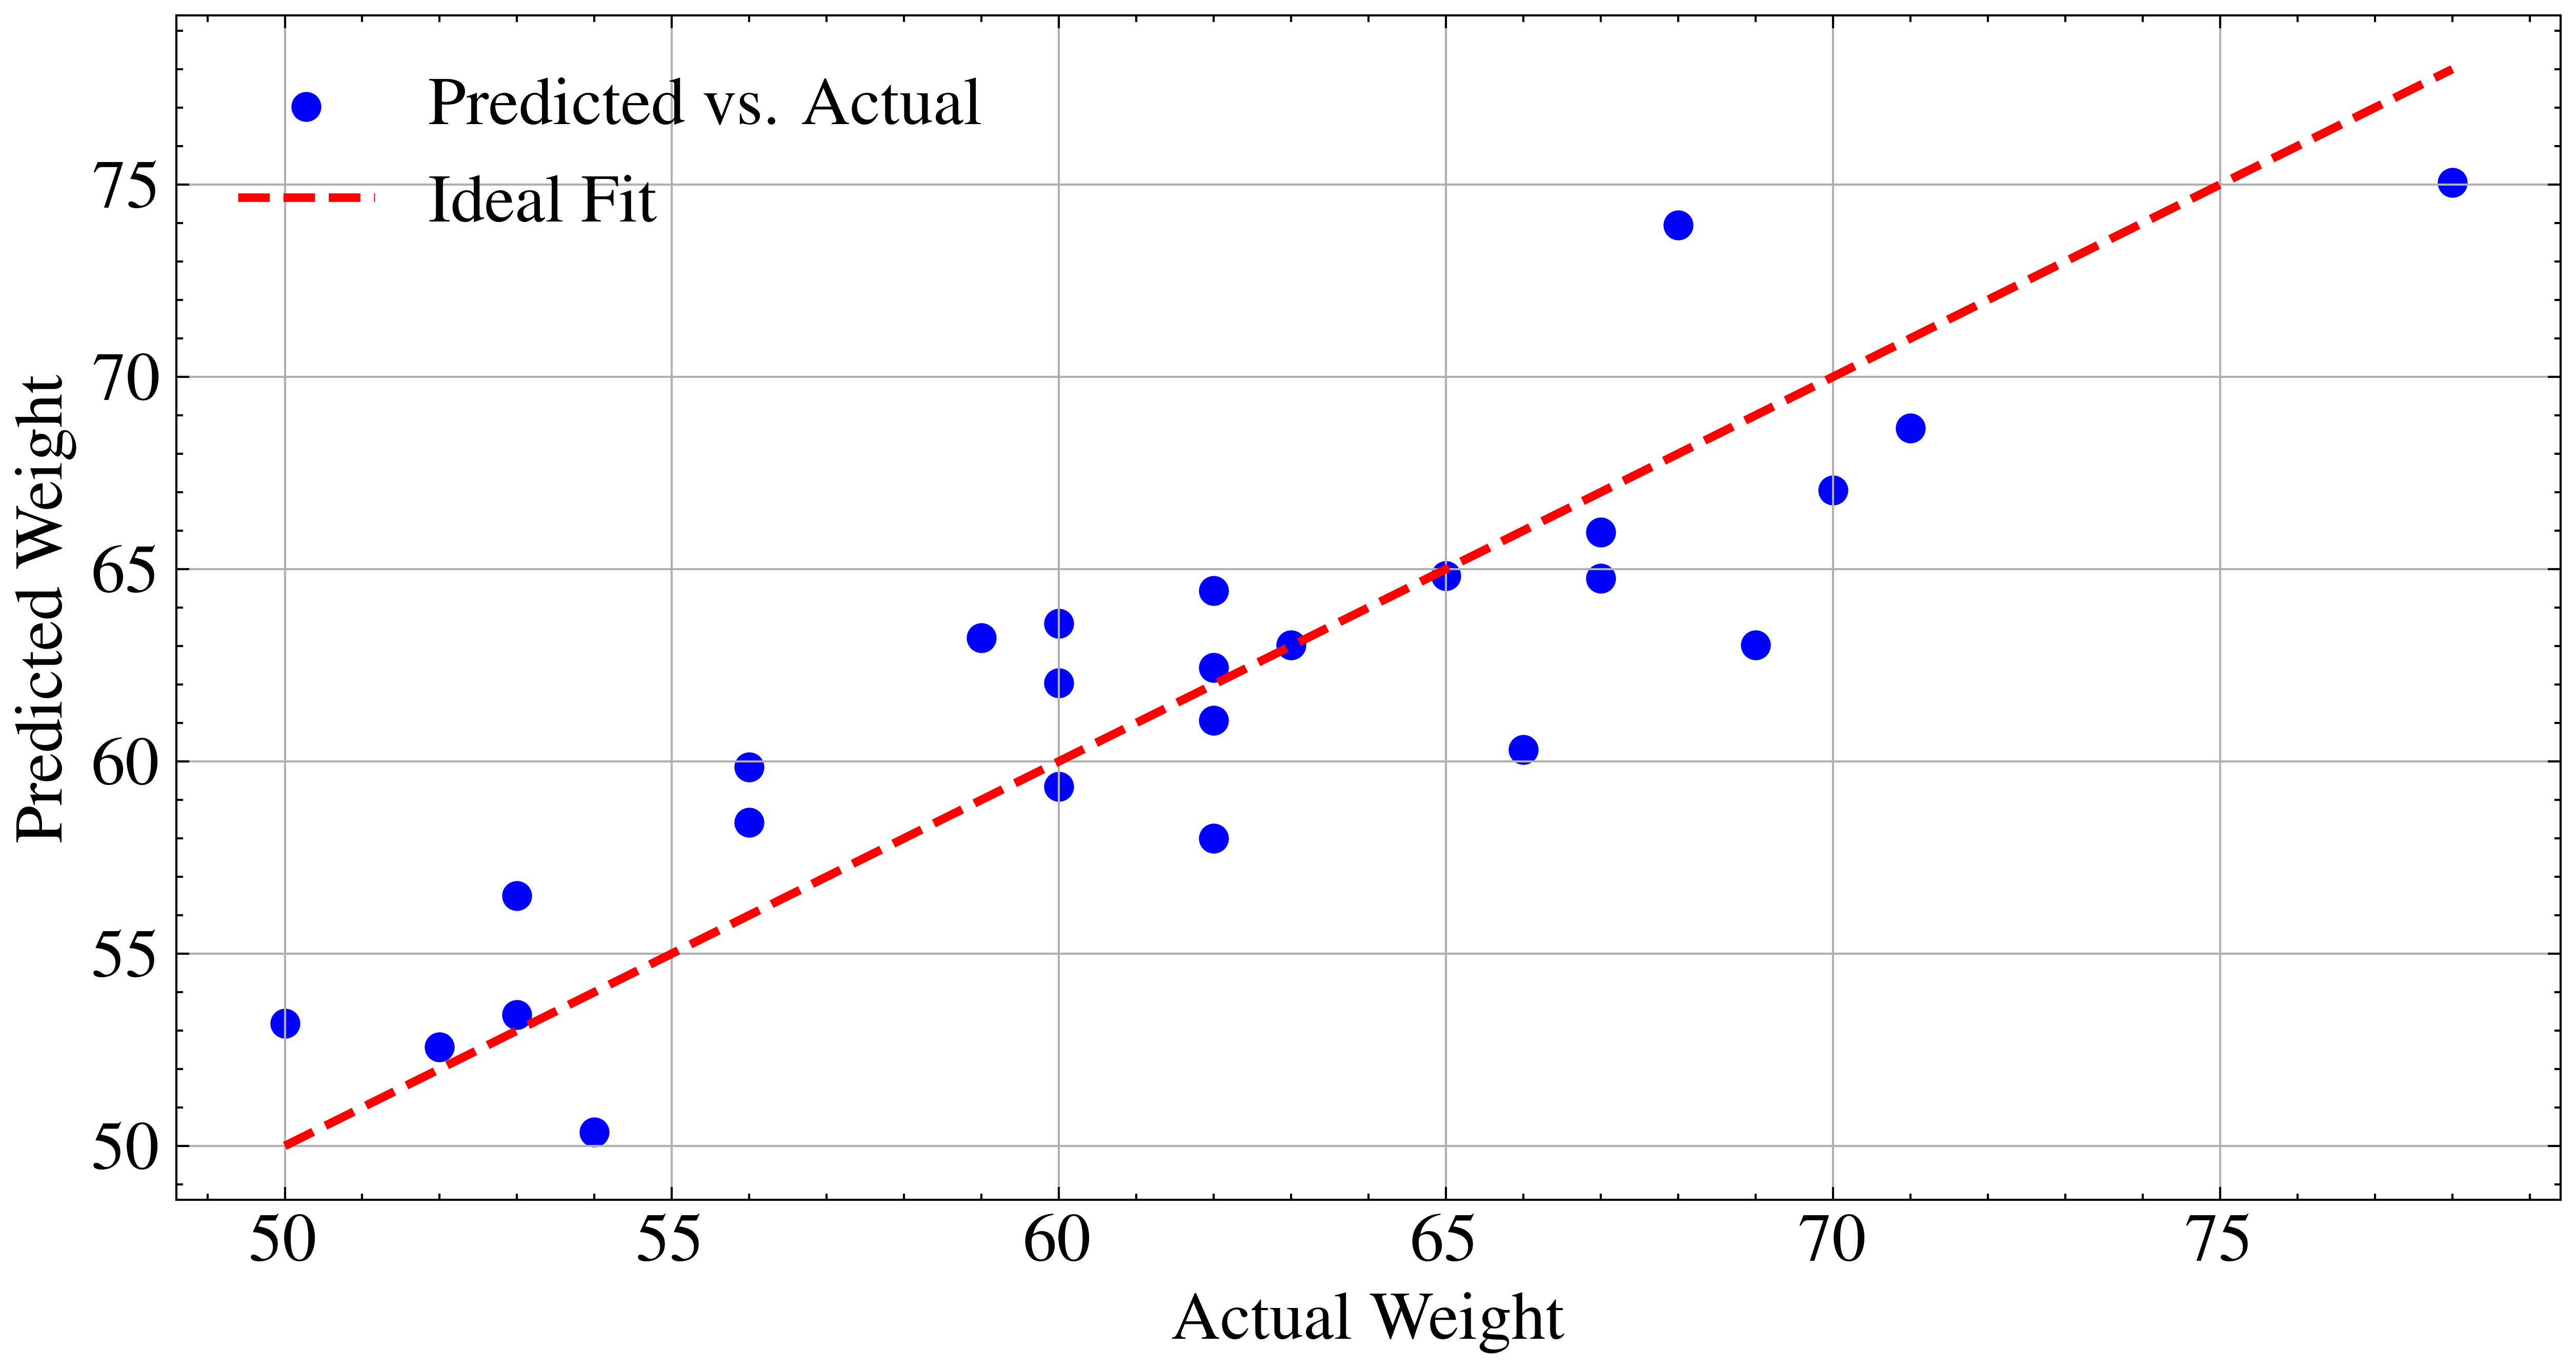
\includegraphics[width=\linewidth]{src/figures/polynominal-regression/polynomial_regression-n-2.png}
        \subcaption{$n=2$}
    \end{subfigure}
    \begin{subfigure}{0.48\linewidth}
        \centering
        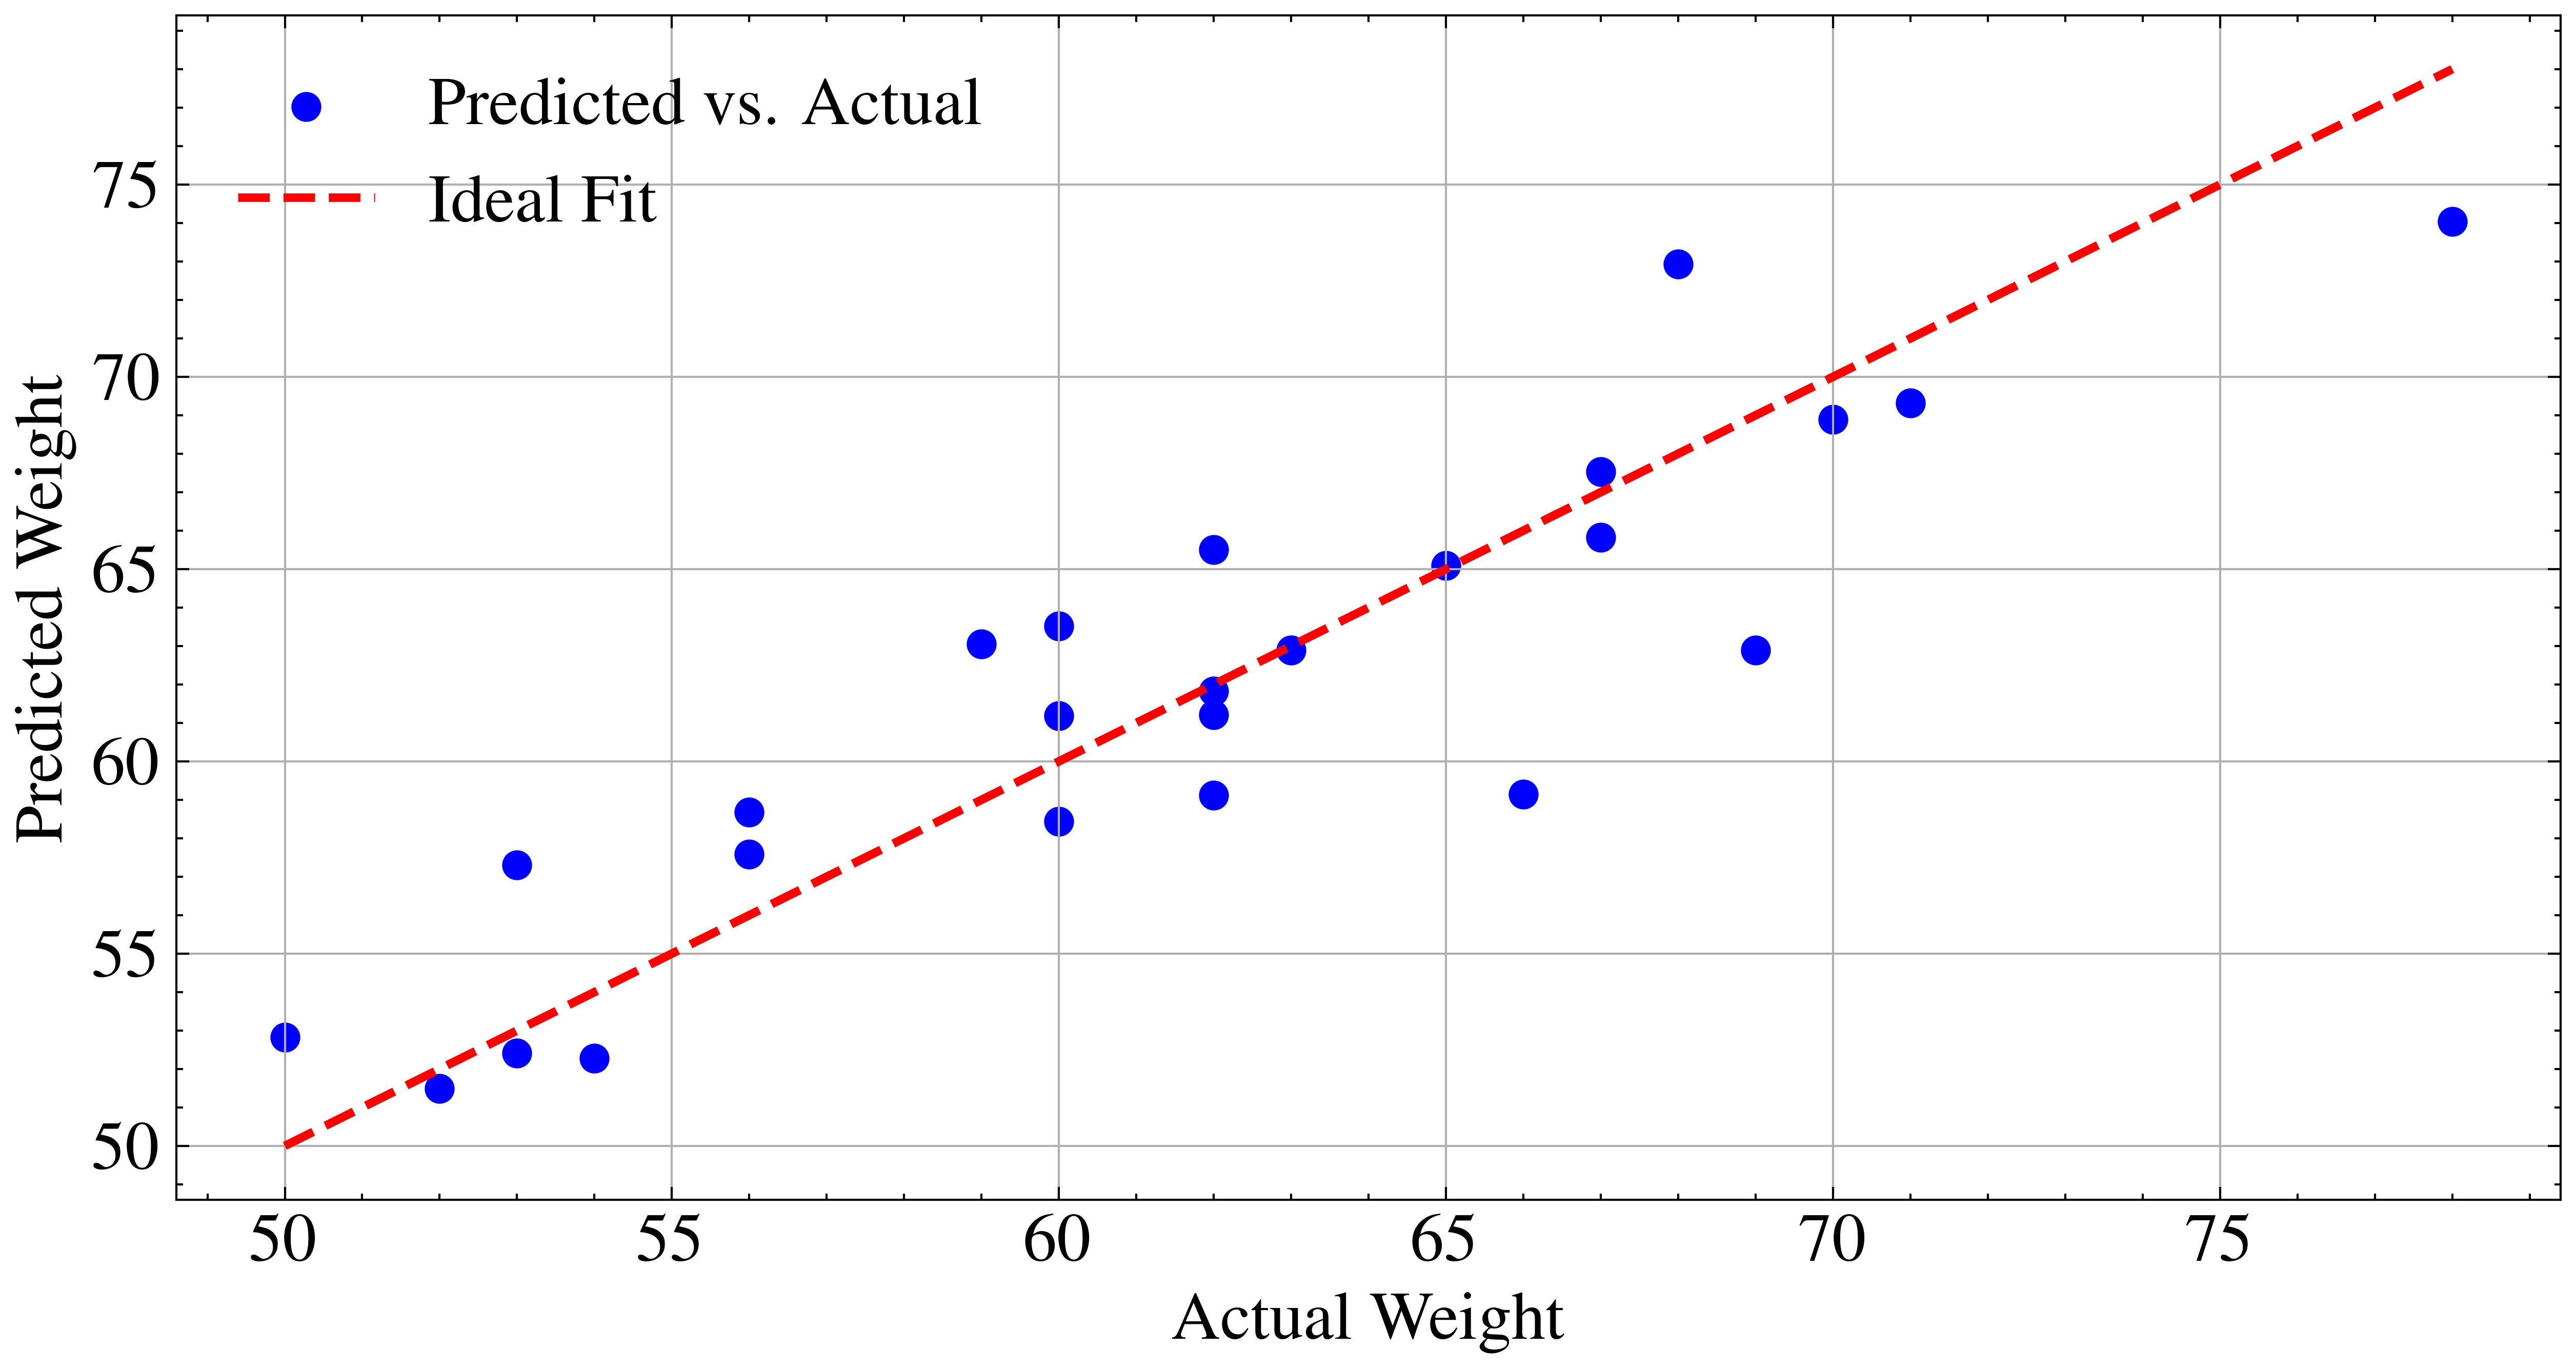
\includegraphics[width=\linewidth]{src/figures/polynominal-regression/polynomial_regression-n-3.png}
        \subcaption{$n=3$}
    \end{subfigure}
    \begin{subfigure}{0.48\linewidth}
        \centering
        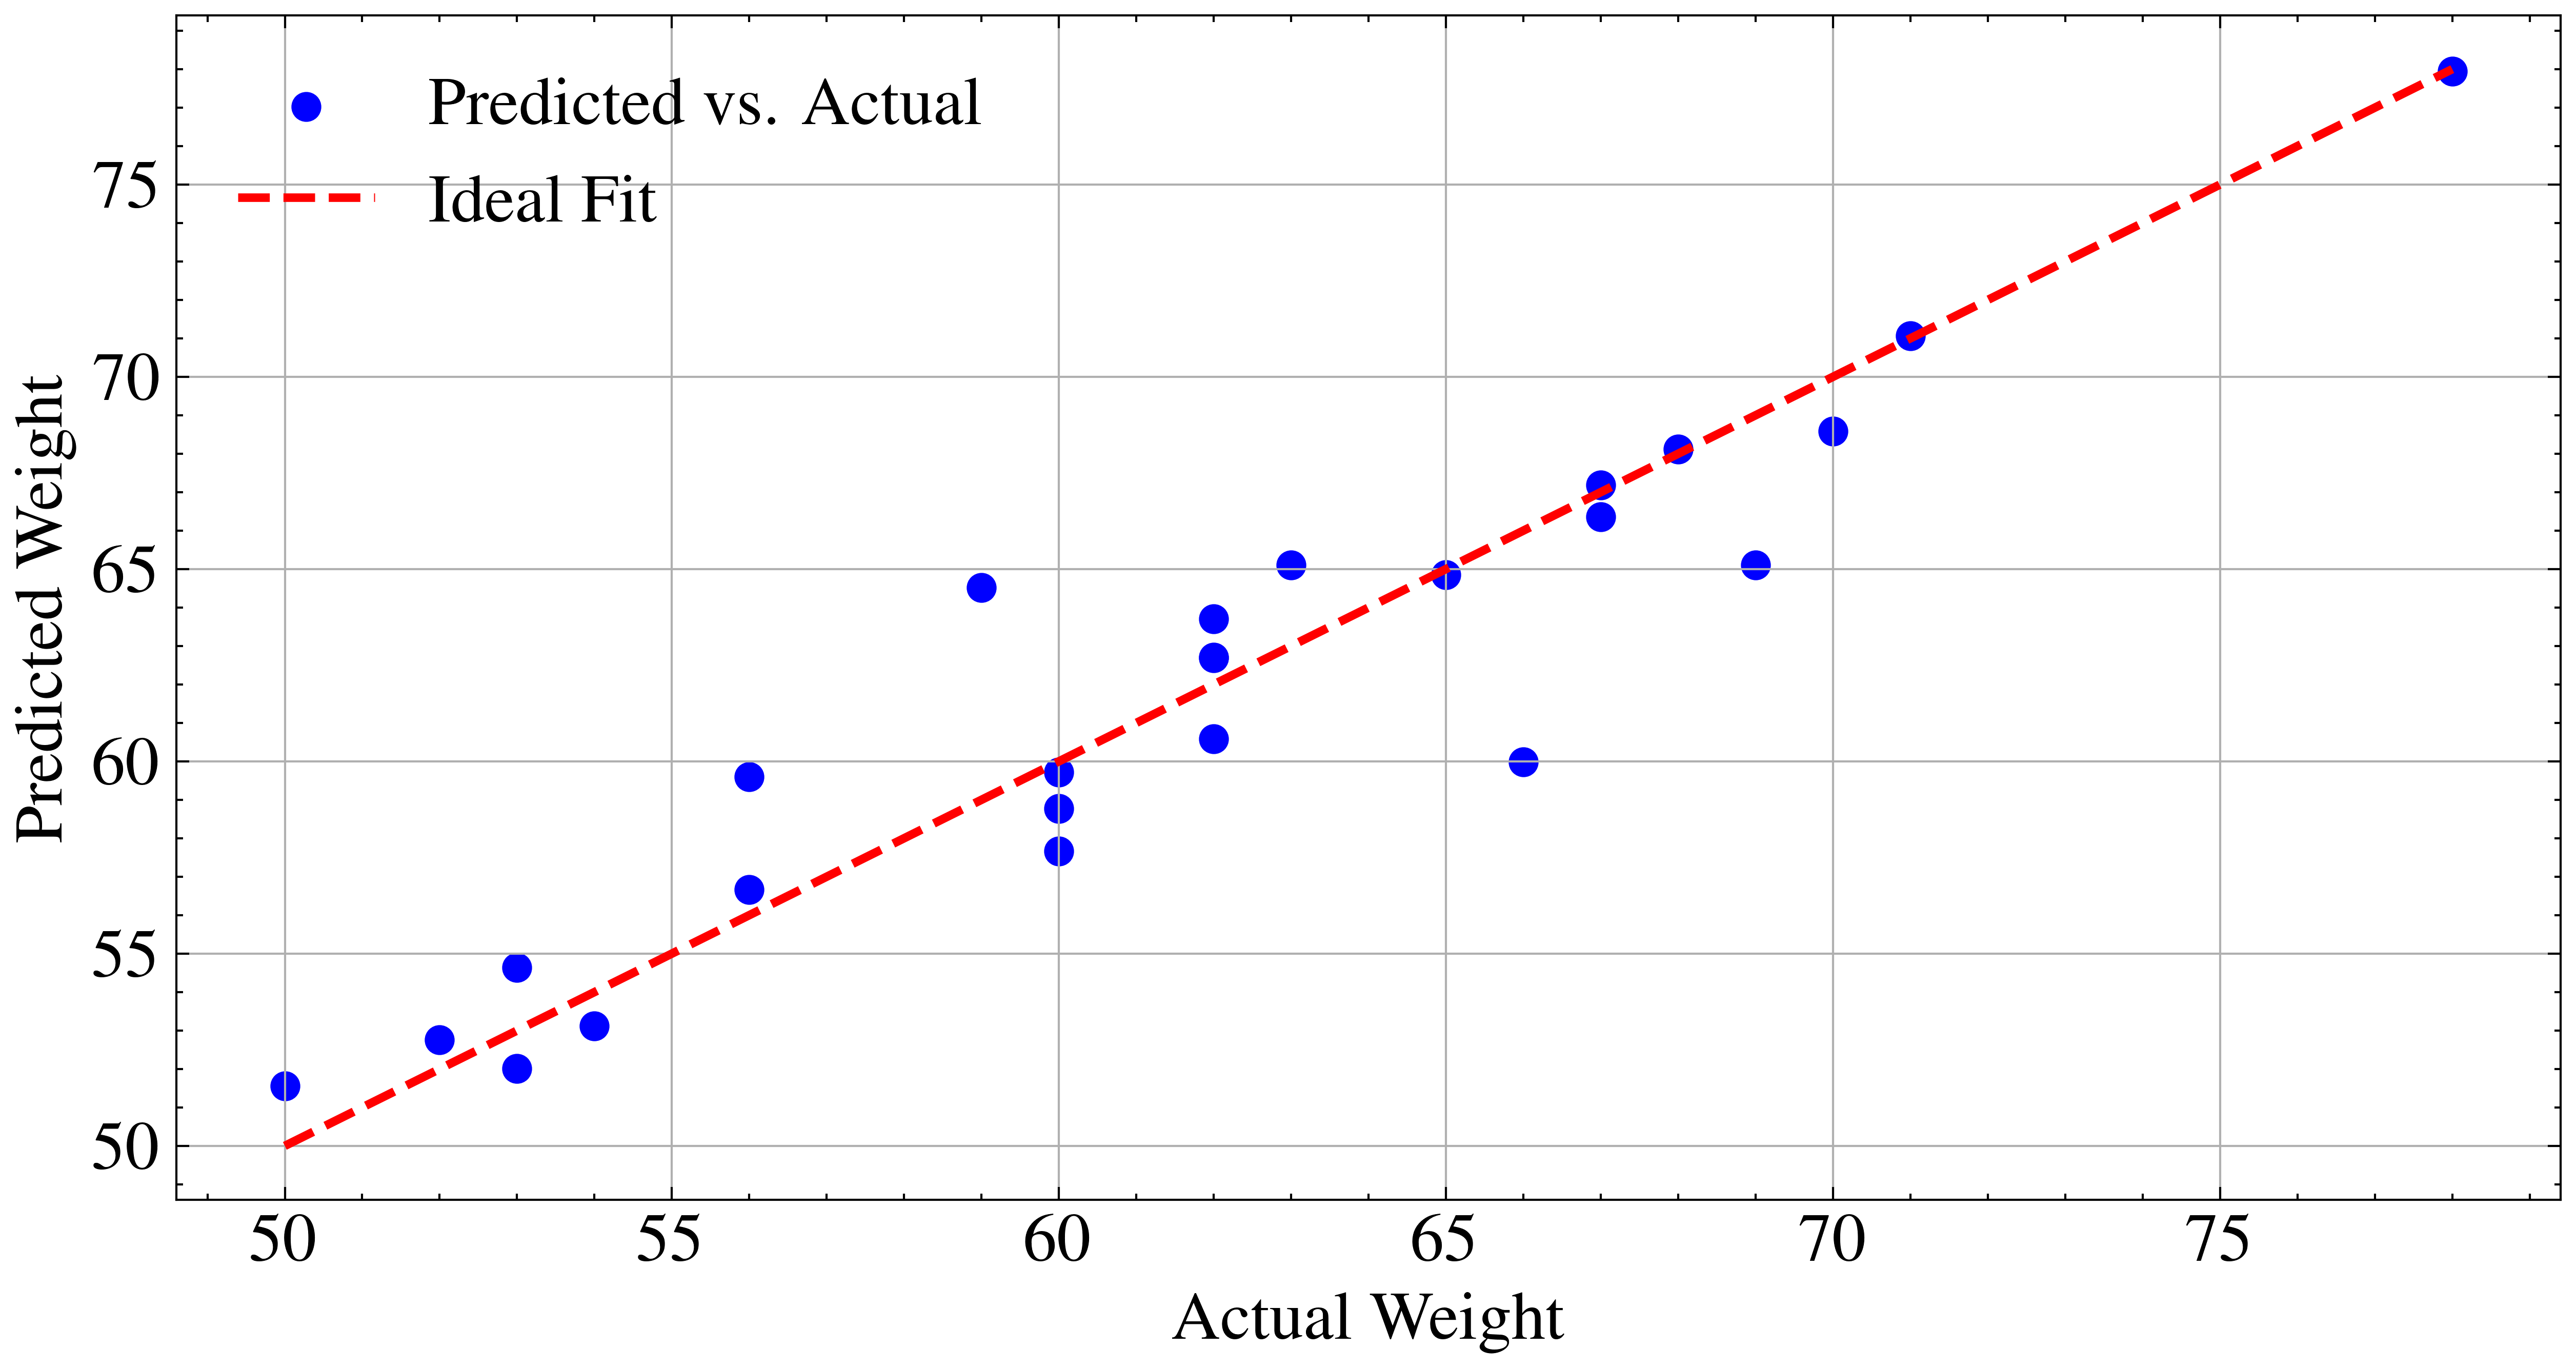
\includegraphics[width=\linewidth]{src/figures/polynominal-regression/polynomial_regression-n-4.png}
        \subcaption{$n=4$}
    \end{subfigure}
    \caption{Polynomial regression with different degrees.}\label{fig:polynomial-regression}
\end{figure}
